\documentclass[10pt,a4paper]{report}
\usepackage{graphicx}
\usepackage{hyperref}
\hypersetup{
    colorlinks=true,
    linkcolor=blue,
    filecolor=magenta,      
    urlcolor=cyan,
}
 
\urlstyle{same}

%\renewcommand{\chaptername}{}
%\renewcommand{\thechapter}{}

\begin{document}

\title{Neural networks for hydraulic drive control}
\author{Alexandre Pascault}
\maketitle
\begin{abstract}
	This document presents the work done during my internship at the Department of Mechatronics from the Warsaw University of Technology.
\end{abstract}

\chapter{System Description}
\label{sec:System Description}

\chapter{Cleaning the data}
\label{sec:Cleaning the data}
\section{The data}
\label{sub:The data}
The data that will be used for the model and offline training has already been collected beforehand. It consists of csv tables containing values for the control command, the position of the hydraulic cylinder, and a PRBS signal that changed every 400ms. All these were collected with a sampling frequency of 1000Hz.
\\
The hydraulic cylinder is controlled by applying a tension between -10V and 10V. This tension dictates the speed of the cylinder on its axis. Since we only have measurements of the position, we need to differentiate those to get the speed of the cylinder as this will be the input data for the classifier. The main issue here is that the position measurements are noisy, to the point that differentiating those directly yield an extremely noisy, barely usable speed signal.

\section{Filtering}
\label{sec:Filtering}

We start by filtering the signal with a 12\textsuperscript{th} order digital low-pass filter with a cutoff frequency of 12Hz. We generate this filter using the python \textit{firwin} function from the \textit{scipy.signal} python library, that computes the filter coefficients using the windowing method. The choice of these parameters was done empirically. 

\begin{figure}[h]
	\begin{center}
		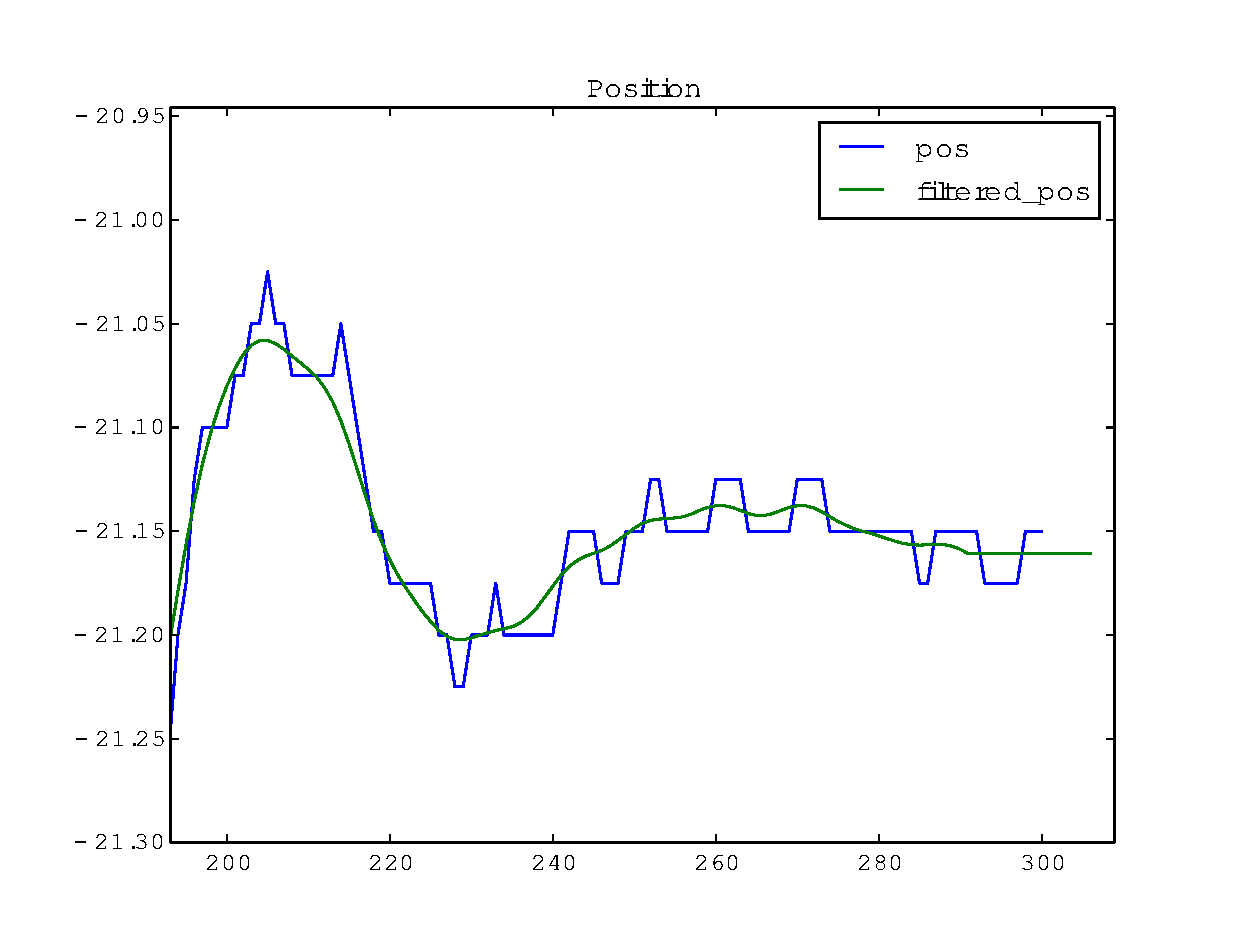
\includegraphics[scale=0.5]{Figures/position.eps}
	\end{center}
	\caption{Raw and filtered position}
	\label{fig:positions}
\end{figure}
\noindent The figure \ref{fig:positions} shows the raw data and the filtered positions.


\section{Differentiating}
\label{sec:Differentiating}
We now need to access the speed of the hydraulic cylinder. We compare different methods of differentiation in order to select the most precise one. Our goal is to minimise the distortion of the signal, as any imprecision here might induce errors in the classification.
\\
We begin by using a central finite difference, plotting the speed versus time computed with accuracy from 2 to 8.
%\begin{example}
\\
\vspace{2in}
\textit{Central finite difference with accuracy of 6:}
\begin{equation}
\label{eq:central_difference}
\dot{x(t)} \simeq \frac{-1}{60} * x(t-3) + \frac{3}{20} * x(t-2) -\frac{3}{4} * x(t-1) + \frac{3}{4} * x(t+1) -\frac{3}{20} * x(t+2) + \frac{1}{60} * x(t+3)
\end{equation}
%\end{example}




\end{document}
